% !TeX root = ../thesis_main.tex

% ---------------------------------------------------
% ----- Chapters of the template
% ----- for Bachelor-, Master thesis and class papers
% ---------------------------------------------------
%  Created by C. Müller-Birn on 2012-08-17, CC-BY-SA 3.0.
%  Freie Universität Berlin, Institute of Computer Science, Human Centered Computing. 
%
% TODO remove 2 - to use auto numbering
\chapter{Implementation and deployment}
\label{chap:impl} 

The phase of implementation and deployment followed an agile development process where changes could be deployed easily to get fast feedback from users.

% \localtableofcontents

\section{Architecture}

Let's start with an overview about the architecture and high level user flows.
There are three software components relevant for a basic interaction with the system: the editor frontend, the editor backend and the \Gls{manager} backend, which is responsible for
authentication, app management and providing dynamic resources as ZIP files.
At the beginning of a user journey, the user logs in at the root domain (e.g. \url{https://builder.purplemanager.com} for production apps).
The authentication details will not be covered here as these would go beyond the scope of a bachelor thesis and are not relevant for the UX.
The \Gls{rest} of the \Gls{manager} and the way dynamic resources get downloaded and merged is one of the basic fixed technical requirements introduced by the surrounding ecosystem.
\\
The UML sequence diagram fig. \ref{fig:userflow} displays a typical interaction of a user with the editor frontend after he selected an app; pulling the latest dynamic resources, editing a file and merging the changes.
\begin{figure}[h!]
  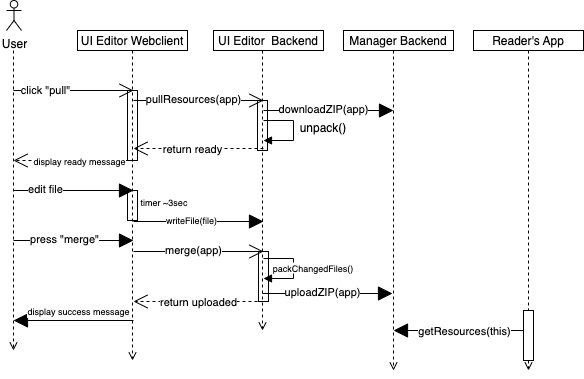
\includegraphics[width=\textwidth]{pics/user-flow.uml.drawio.png}
  \caption{A typical interaction of a user with the UI Editor frontend and it's dependencies}
  \label{fig:userflow}
\end{figure}
\pagebreak
\section{Software stack}
From a company's perspective, it is advantageous to keep the technology stack as narrow as possible.
For this case study, the most important point was the availability of additional personnel with knowledge about the frameworks and languages used.
To conform with the company's \Gls{devops} practices the only requirement is to run the project inside Docker containers in a \Gls{kubernetes} environment.
\\\\
For this project the Typescript language (\url{https://www.typescriptlang.org}) is used on back- and frontend.
The advantage is the availability of many skilled personnel in the company as well as an established ecosystem and easy sharing of code and type definitions between frontend and backend.
\\
The rest of the software stack is fairly common in today's web development industry too:

\begin{description}
  \item[Frontend] \leavevmode
  \begin{description}
    \item[Rendering framework] \textit{React JS v18} (\url{https://reactjs.org/})
    \item[UI Component Library] \textit{Blueprint JS} (\url{https://blueprintjs.com/}) provides components so a consistent design system with common functionality like buttons, dropdowns, filters etc. can be used.
    \item[Other libraries] \textit{ReactQuery / TanQuery} to manage, cache and invalidate HTTP API requests to the backend, \textit{Zustand JS} for shared reactive state management and \textit{Zod} for type validation at runtime.
  \end{description}
  \item[Backend] \leavevmode
  \begin{description}
    \item[HTTP Server] Express on Node JS, which is the most common combination to run an JavaScript based HTTP server (see \cite{Github:VanoDevium/node-framework-stars}).
    \item[Routing abstraction] TSOA (\url{https://github.com/lukeautry/tsoa}) on top of Express, which is a Typescript library to provide Java-Spring like syntax with controllers, dependency injection and parameter validation at runtime.
  \end{description}
  \item[Testing] using Vitest (\url{https://vitest.dev/}) for Unit tests and Playwright (\url{https://playwright.dev/}) as E2E test runtime. 
  \item[DevOps] Gitlab Pipelines to build, test and package on every merge request or commit to develop and master branch.
  \item[Project Setup] Monorepository with PNPM as package manager and Turborepo to manage package dependencies and automatic optimal build scheduling and caching.
\end{description}

\section{CI/CD}

Continuous Integration and Continuous Delivery, short CI/CD, a core practice of agile software development, enables fast release and deployment cycles which is crucial for agile prototyping and development.
A Gitlab CI/CD Pipeline was set up for the UI builder, consisting of Build, Package, and Deploy stages.
The Build stage also executed unit and end-to-end tests due to technical reasons for efficiency.\\
Having a fast and reliable CI/CD process during development and prototyping was valuable, as it allowed for quick reactions to user input and deployment to a staging domain for user feedback in under 10 minutes.
Separating staging and production systems also allowed for more confident deployment of quick fixes for validation in a production-like environment without interrupting users.

\section{Feature examples}

A selection of features is presented that were implemented during the UI Editor case study is presented in the following section.
These features are chosen as examples to how the HCI methods and outcomes from the user research phase influenced their design and how they can improve the user's experience with the tool. 

\subsection{File management - open multiple files as tabs}

A common workflow consists of editing multiple files simultaneously, for example having the view configuration open while adding translations for newly added components.
The old editor tool allowed to only open one file at a time, which got closed when the user opened another file. This showed up as a big slowdown during the moderated observation.
All participants mentioned they have to work on multiple files and that they are annoyed by the workflow, especially when opening large view configs can take more than 30 seconds.
\\
The solution was inspired by the file management that most \Gls{ide}s provide; a bar on top where all the opened files are listed and the user can quickly switch between them or close the ones not needed (see fig. \ref{fig:file-tabs}). 

\begin{figure}[h!]
  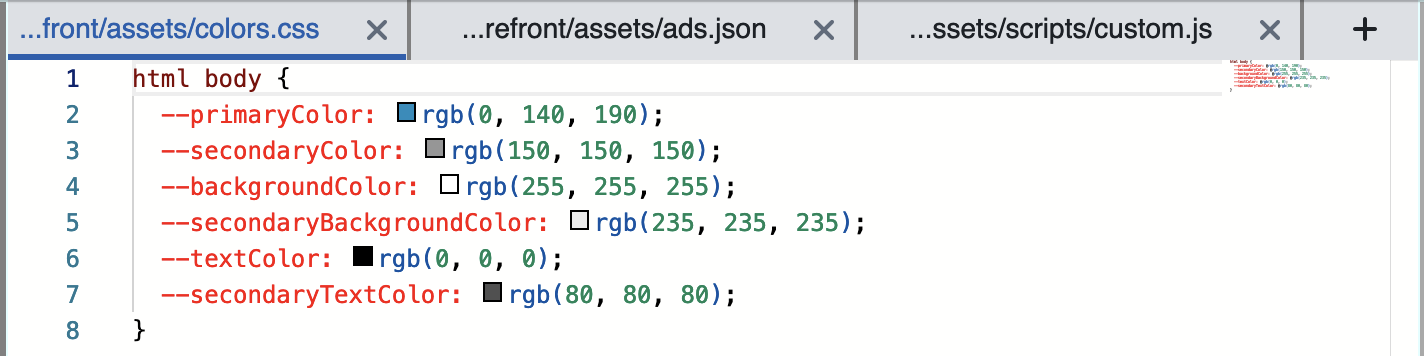
\includegraphics[width=\textwidth]{pics/file_tabs.png}
  \caption{Screenshot of the latest iteration of file tabs}
  \label{fig:file-tabs}
\end{figure}

\subsection{File management - quick links}

A second feature regarding the file management is ``quick links''. While all target groups benefit from this, especially for the personas \textit{Steffi, \ref{subsec:persona:productdev}} and \textit{Karsten, \ref{subsec:persona:itpublishing}}
this can speed up common tasks considerably.

The basic idea is to bookmark commonly used files, e.g. the translation or ad config, and have them prominently available when opening a new app.
For the implementation, three factors needed to be considered:
\begin{description}
  \item[Where to save?] The quick links are stored in the \Gls{localstorage} of the user's browser, so the list is available across apps.
  \item[How to manage?] The user has a list on the settings view, where entries can be added, deleted and changed, but the file path needs to be inserted manually. To enhance the user experience, a proposal exists to either add a file picker in the settings or add a bookmark button to the file manager.
  \item[How to present the links?] The links must be easily accessible to provide the intended benefit. The solution was to show them prominently when entering the \textit{edit} view and no file was opened yet.
  In addition, the UI shows if the link points to a file, which gets opened as a new file tab, to a folder which will navigate the file explorer there, or if the path doesn't exist in the current app.
  \begin{figure}[h!]
    \centering
    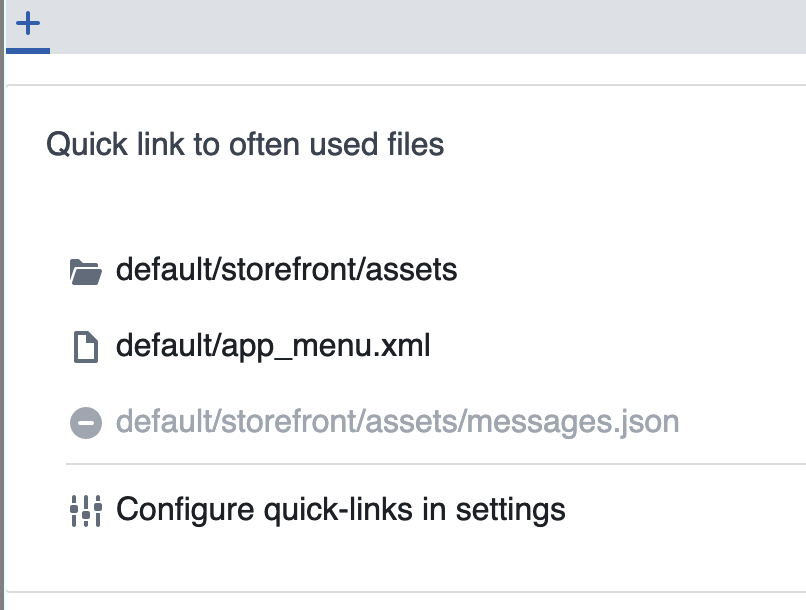
\includegraphics[width=0.4\textwidth]{pics/quick_links.png}
    \caption{The three types of quick links: Folder, file and not available}
  \end{figure}
\end{description}

\subsection{Editor - Abstraction to provide per-file custom editors}

Purple Experience relies on a variety of configuration files, all with different schemata and functional intents.
To provide an efficient and error reduced workflow to users, it is important to have specialized file editors.

For view configurations for example, the JSON Editor Library (\url{https://github.com/json-editor/json-editor}) is used, combined with the generated JSON Schema files. For the translations there exists a custom editor that has a fuzzy search function and makes it easy to manage translation entries.

The abstraction is done solely in the frontend and follows React's ``\Gls{comp-over-inh}'' pattern and can be seen in fig. \ref{fig:abstract-editor}.
To add a new specialized editor the only two steps are creating a new functional component that implements the \textit{EditorImpl} interface
and add that editor in the \textit{EditorRegistry} to get returned for the file paths in question.
\\\\
\begin{figure}[h!]
  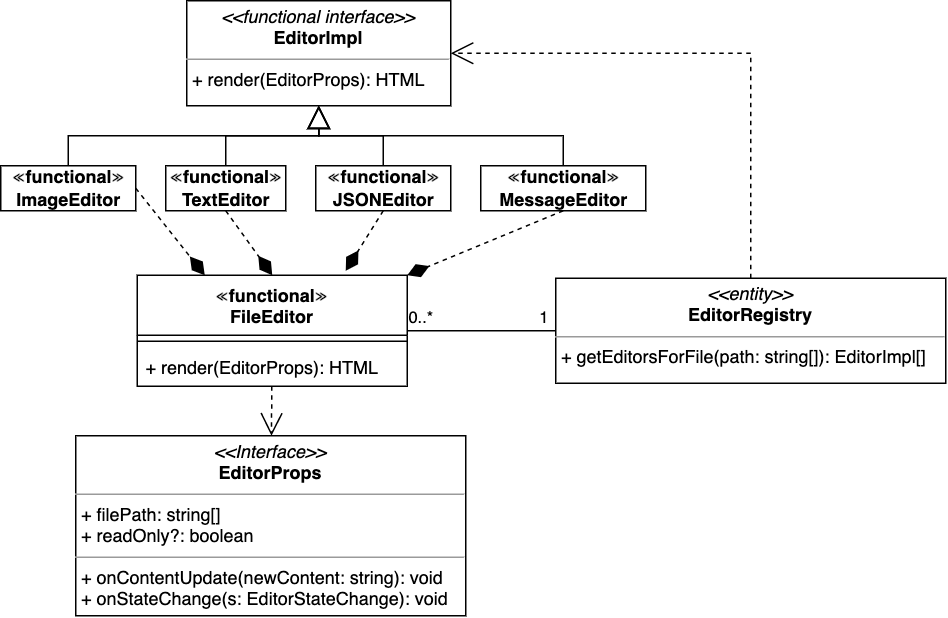
\includegraphics[width=\textwidth]{pics/abstract_editor_uml.drawio.png}
  \caption{Class diagram showing the editor abstraction in React JS. Due to modern React JS architecture, component classes are replaced with functional components (marked with $\ll functional\gg$).}
  \label{fig:abstract-editor}
\end{figure}
Examples of custom editor implementations can be seen in Appendix \ref{fig:messages_editor} and \ref{fig:ads-editor}.


\section{Automated Testing}
\label{sec:automated-testing}

As already elaborated, fast CI/CD pipelines plays a crucial role for agile prototyping and development.
Automated tests in turn contribute to the confidence of developers to deploy more frequently and can reduce load from the QA team to test standard workflows every time a new release is planned.
For the Experience Builder two of the most common testing levels are used: unit tests and End-to-End tests (also known as E2E or System tests).
\\\\
Unit tests are mostly used to test one ``component'' in a sandboxed environment, in practice often done per-function or per-class.
On the client, the distinction is between testing of UI components and business logic code that is encapsulated in classes or JavaScript modules.

Unit tests also are helpful during development to test software patterns before doing large refactorings and to do test-driven development (TDD), where the specifications and constraints can be laid out as code with invariants, pre- and postconditions.
Then the implementation is done while continuously running the tests again until they don't fail anymore.
\\
For TDD as well as CI/CD Pipelines, the speed of the test execution is important. If a single test run takes multiple minutes, the developer is blocked during that time and can't progress on the task.
Therefore, the aim was to achieve the shortest possible runtime, compatible with UI- / browser testing as well as Node JS for the server code.
After evaluating commonly used frameworks, Vitest (\url{https://vitest.dev/}) was chosen, which fullfills all the requirements, is compatible with our build tools and runs tests in parallel if possible. The Unit test suites can be hot-reloaded and reexecuted on change in less than a second, which is a nice developer experience.
\\\\
Due to the complexity of interoperation between components, APIs and the Web standards, unit tests alone are not enough to guarantee the different modules work together as expected. 
\\
E2E tests are supposed to cover a typical user interaction with the service to validate the interaction between business logic components, UI and the user itself.
First a headless browser\footnote{Headless browsers are browser instances that don't render the actual content to a user's screen, but run as a CLI application and still execute all JavaScript, CSS and HTML.} (\url{https://pptr.dev/}) was used in combination with Vitest,
but writing and debugging tests proved to be slow and error-prone.
\\\\
Later in the process, the E2E tests were rewritten for an alternative test framework called Playwright (\url{https://playwright.dev/}), which allows recording a test case in a normal browser window and then generates the test code automatically, allowing to be adapted and generalized if needed.
After the tests were ported to the new framework developers can enjoy better debugging tools and the ability to add new tests easier.
\\
This can be an example for others, that investing time to investigate new tools and port code to them if they bring value can improve developer experience and thus also speed and confidence.

\section{Privacy-friendly analytics \& monitoring}
\label{sec:analytics}

Sooner or later, you find yourself in a pickle when it comes to tracking.
On the one hand, the data can provide valuable insights into the behavior of many users, which would not be possible through qualitative research.
On the other hand, the most common tools like Google Analytics track users with cookies, which creates new challenges regarding GDPR compliance.
\\\\
The Purple product owner showed me a SaaS called \url{https://squeaky.ai/}, which is a cookieless solution to track users on this page.
While it can't provide the same level of demographic information a cookie based solution can, it still collects the most important data like usage statistics,
user interactions, occurred JavaScript errors and can even show heatmaps per page to visualize which UI elements the user interacts with the most.

\begin{figure}[h]
  \centering
  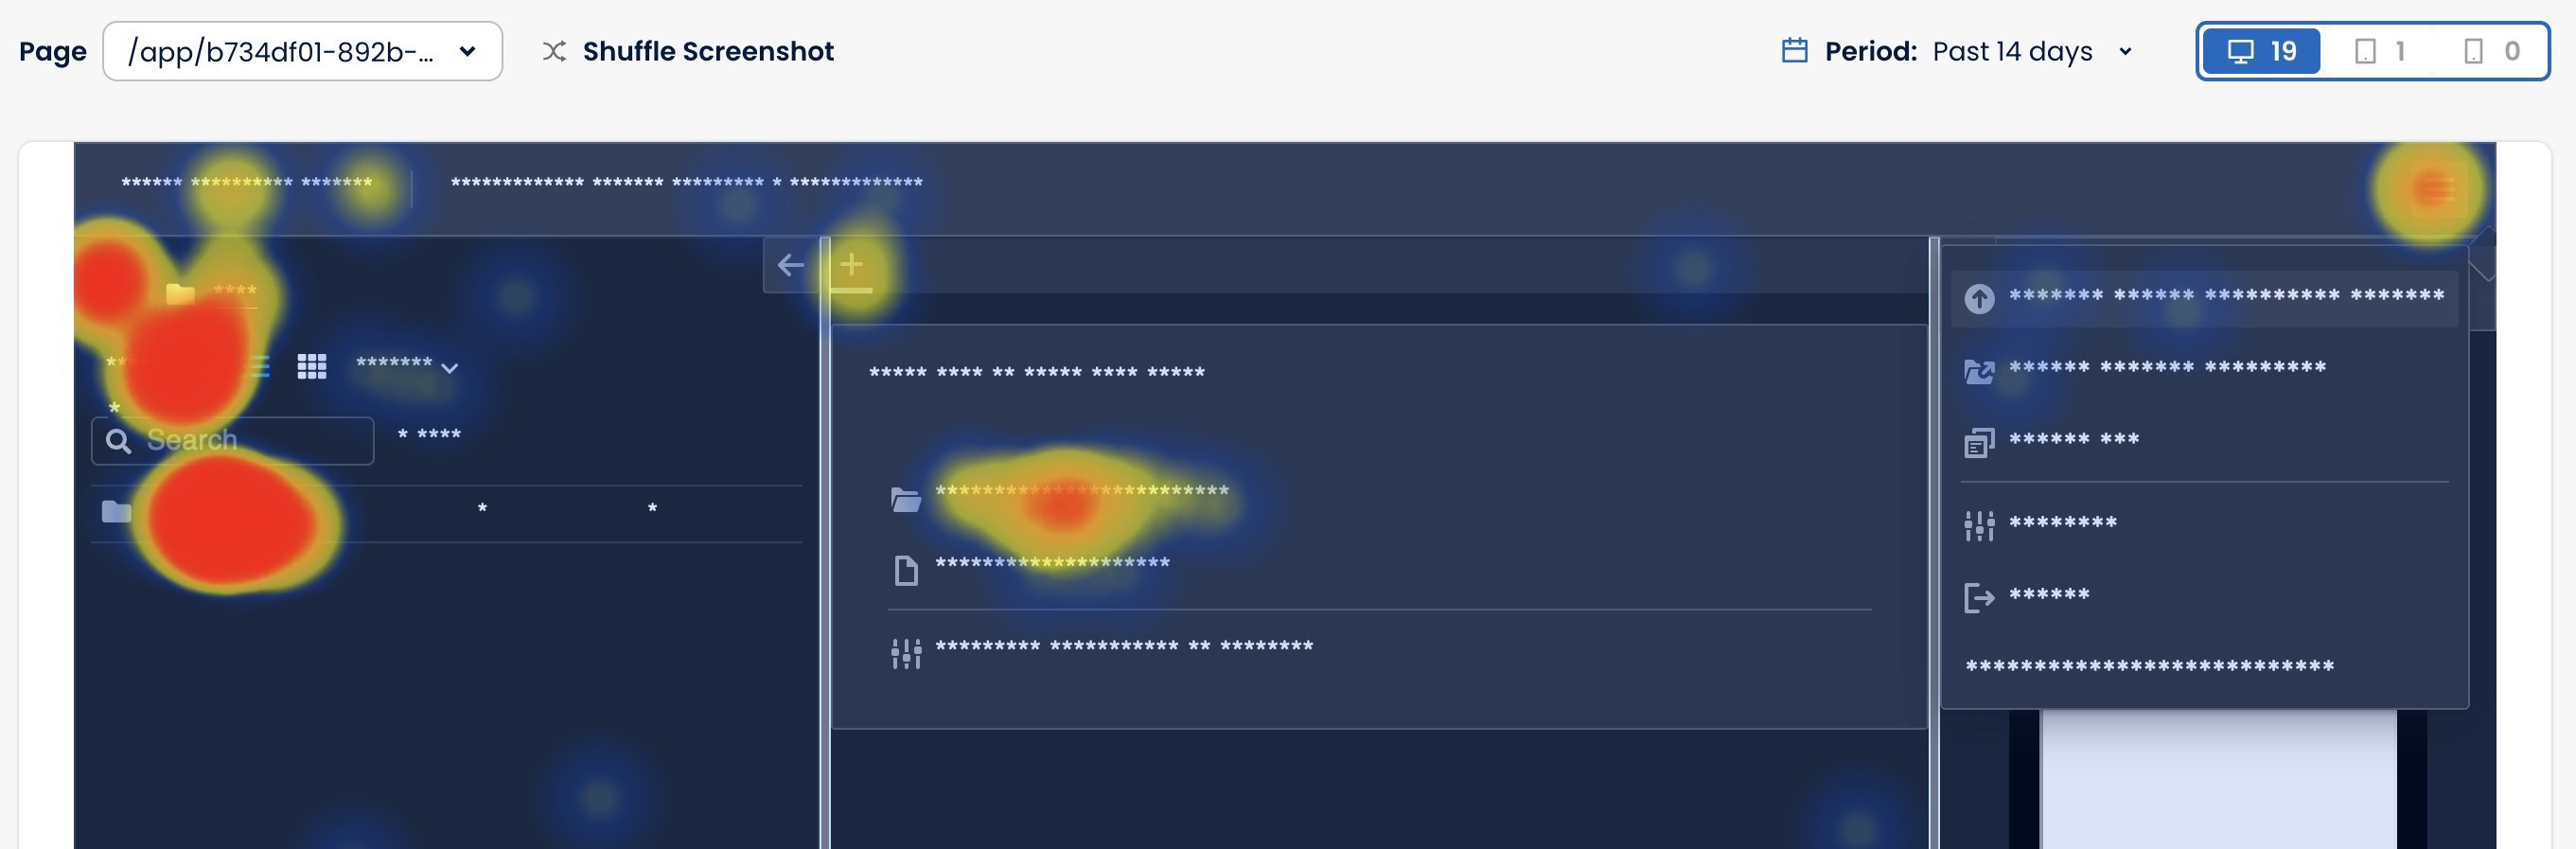
\includegraphics[width=0.75\textwidth]{pics/squeaky_heatmap.jpg}
  \caption{Screenshot: Squeaky.ai heatmap of an app's edit view}
  \label{fig:squeaky}
\end{figure}

These heatmaps for example can show if a new UI feature is used by users and how they interact with the page in general.
Fig. \ref{fig:squeaky} shows that the users mostly interacted with the file explorer and only did a few clicks in the editor panel.

To analyze the usage growth, fig. \ref{fig:squeaky_users} indicates how the number of page views per week increased steadily since the internal beta was launched (except for the dip during the Christmas holidays).
The graph clearly shows that the time-bound goal from the SMART goals (\ref{fig:smart}) has been successfully achieved.

\begin{figure}[h]
  \centering
  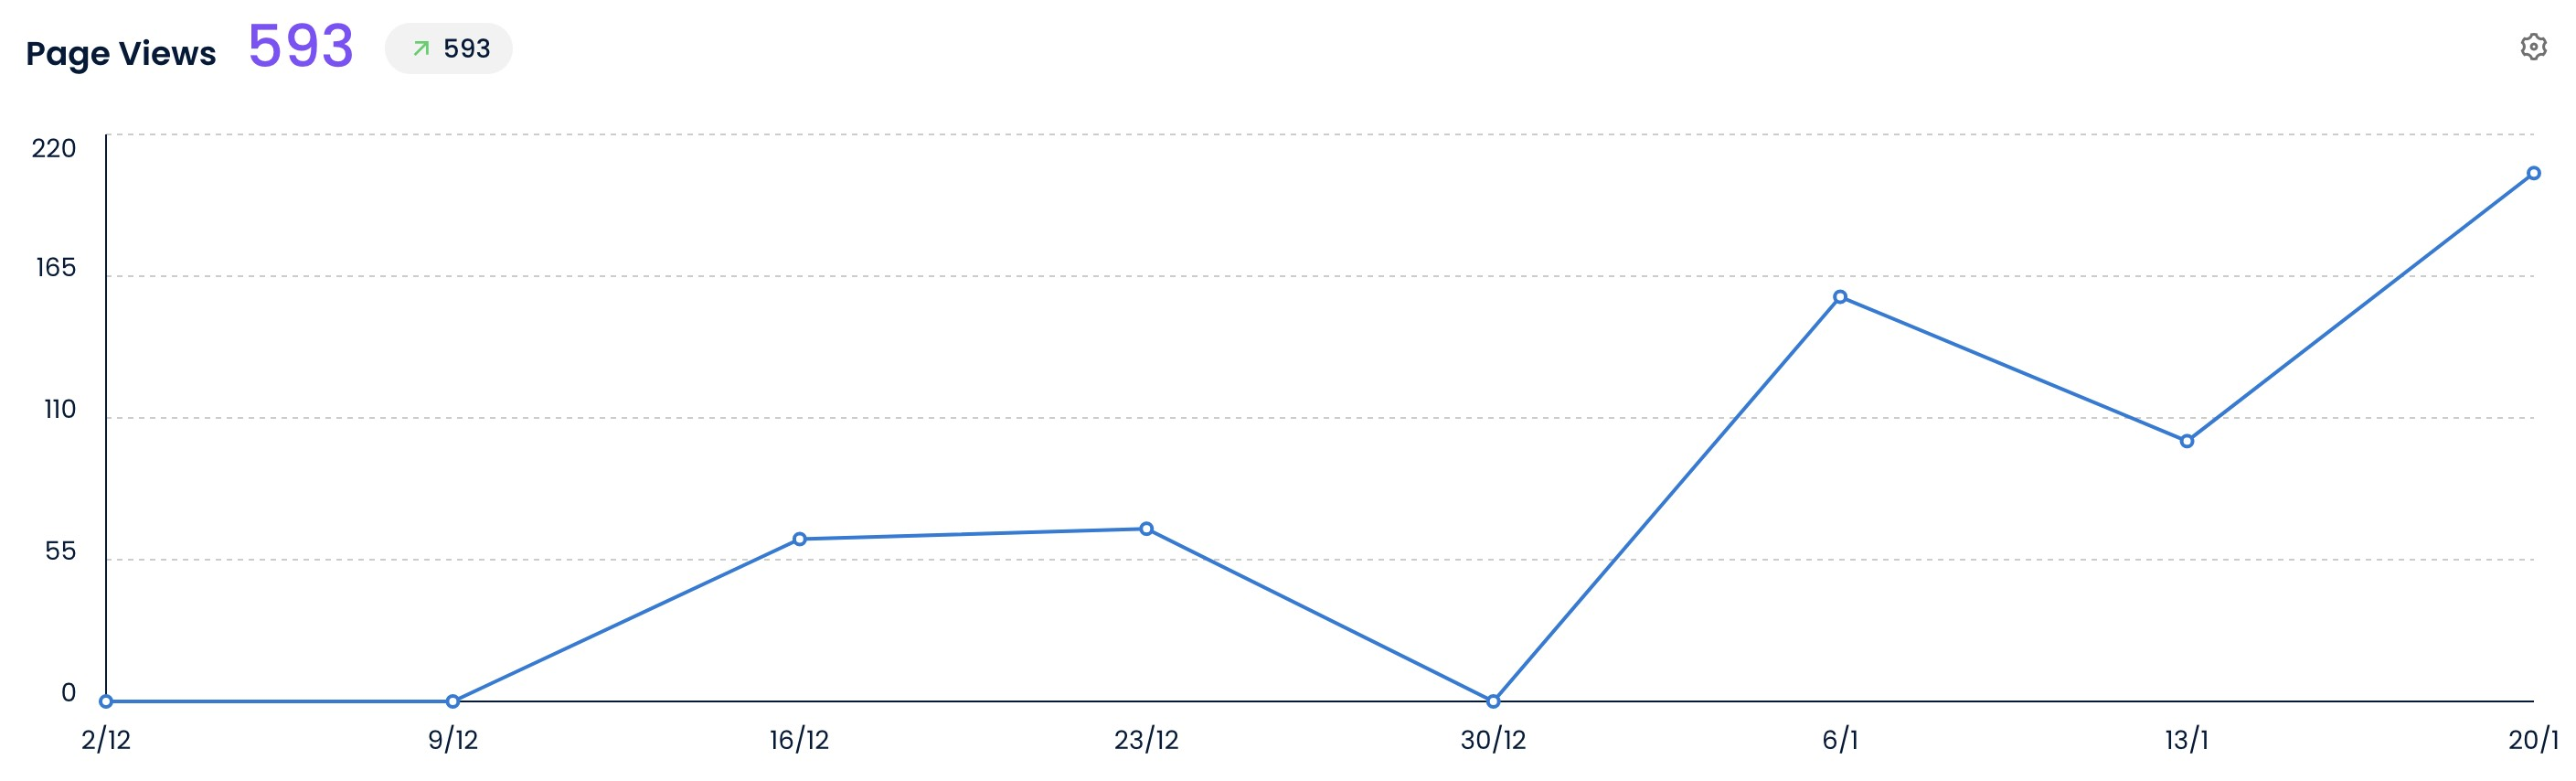
\includegraphics[width=\textwidth]{pics/squeaky_user_curve.jpg}
  \caption{Screenshot: Squeaky.ai page views since December 2022}
  \label{fig:squeaky_users}
\end{figure}

\section{User Testing, Feedback, Beta and Monitoring}

After a first stable deployment was available for stating and production dynamic resources and all basic requirements were met, the user tests for the Beta-phase started.
Four people from our company agreed to try to use the editor and give verbal feedback. Three of them were already participants of the interviews.

The reported bugs were and still will be written into Jira tickets so the status can be properly tracked and release notes can be easier generated.
Mostly the bugs were edge cases where a file wouldn't open or the changes were not saved properly.


\section{Communication and Documentation}
Communicating with the test users and documenting the technical aspects of the software, the progress and how to use certain features is
another building block towards a good user- and developer experience.
\\
For the communication, a Microsoft Teams Channel was utilized, a group chat where all invited persons (in case of the internal Beta-phase company-wide) can write with each other and create posts.
This was used for notifications about new deployments and if in the aftermath someone found a bug that could affect multiple people.

Even though this adds a bit overhead, it proved easier than having everyone write bug tickets directly, as user often don't know how to describe the problem which leads to unclear descriptions, wrong tags and duplicate tickets.
Instead, a developer with knowledge about the system looked at the reports and created a new ticket if the problem was new, otherwise referenced an existing ticket or forwarded the problem to the responsible team.
Jira tickets were all assigned to the UI builder component as well as specific releases so everyone can see with one click which changes and fixes are contained in which release.
\\\\
For the feature documentation, Sprylab uses Confluence for internal documentation and Archbee for external documentation that customers can access too.
As we have the common problem of documentation getting postponed indefinitely, I tried to integrate writing documentation directly int o the development flow and only close a ticket if the documentation
was written and reviewed by one additional person. Due to time and personnel shortages, this was unfortunately not always possible and will require more future attention.

